\documentclass[12pt,a4paper]{extreport}
\usepackage[a4paper, top=1.5cm, bottom=1.5cm, left=1.5cm, right=1.5cm]{geometry}
\setlength{\parindent}{1.25cm} % Отступ красной строки
\usepackage{listings}
\usepackage{caption}

\usepackage{hyperref}
\usepackage{booktabs}
\usepackage{lipsum}

\usepackage[frak=esstix]{mathalpha} % красивый готический шрифт.

\usepackage{graphicx} % Для того, чтобы вставлять картинки.
\usepackage{wrapfig} % Картинка, обтекаемая текстом.
\usepackage{amssymb}
\usepackage{amsmath} % Чтобы вставлять обычный текст в формулу с помощью \text. Фигурная скобка в системе уравнений.

\usepackage{multicol} % Для написания текста в несколько колонок

\usepackage{setspace} % Для изменения межстрочного интервала внутри текста. \begin{spacing}{0.8}.

\usepackage{float} % Чтобы была опция таблиц H, запрещающая им бегать по документу
\restylefloat{table}

\usepackage{gensymb} % Геометрические символы. (градусы \degree)..

\usepackage[warn]{mathtext} % Русские символы в формулах. Нужно писать до пакета babel. Указывает, что в формулах используются символы кириллицы, которые по умолчанию печатаются прямым шрифтом.

\usepackage[T2A]{fontenc} % Установить кодировку шрифта для отображения кириллицы в формулах.
\usepackage[utf8]{inputenc}

\usepackage[russian]{babel} % Для переноса текста. Нельзя указывать одновременно russian и english, так как использует язык, который стоит правее.

\usepackage{indentfirst} % Красная строка в первом абзаце.

\usepackage{comment} % Для многострочный комментариев.

%\DeclareSymbolFont{T2Aletters}{T2A}{cmr}{m}{it} % Сделать так, чтобы кириллица в формулах печаталась курсивом

\linespread{1.25} % Межстрочный интервал. По умолчанию 1.0

% Объявляем новую команду для переноса строки внутри ячейки таблицы
\newcommand{\specialcell}[2][c]{%
	\begin{tabular}[#1]{@{}c@{}}#2\end{tabular}}

\newcommand{\figref}[1]{(см. рис. \ref{#1})}
\newcommand{\e}[1]{\text{$\cdot10^{#1}$}}
\newcommand{\sigoper}{\hat{\Lambda}}
\renewcommand{\vec}[1]{\boldsymbol{#1}}

\begin{document}
	
	\begin{center}
		\large
		\textsc{Лабораторная работа №3.5.1}
		
		\LARGE
		\textbf{\textsc{Исследование плазмы газового разряда в неоне}}
		\\[5mm]
		
		\large
		Симанкович Александр\\
		Маслов Артём\\
		Б01-104
		\\[3mm]
		03.11.2022
	\end{center}
	
	\section*{Аннотация}

В работе исследуется распределение переменного магнитного поля в полом медном цилиндре.

\textbf{Ключевые слова:} переменное магнитное поле, скин-эффект.
	
	\section*{Введение}

Вещество может находиться в трёх агрегатных состояниях - твёрдом, жидком и газообразном, причём эти состояния последовательно сменяются по мере возрастания температуры. Если и дальше нагревать газ, то сначала молекулы диссоциируют на атомы, а затем и атомы распадаются на электроны и ионы, так что газ становится ионизованным, представляя собой смесь из свободных электронов и ионов, а также нейтральных частиц. Если степень ионизации газа (отношение числа ионизованных атомов к их полному числу) оказывается достаточно велика, то такой газ может обладать качественно новыми свойствами. Поведение заряженных частиц приобретает коллективный характер, так что описание свойств среды не может быть сведено к описанию обычного газа, содержащего некоторое количество отдельных заряженных частиц. Такое состояние ионизованного газа называется \textit{плазмой}.
	
	\section*{Теория}

\subsection*{Уравнение колебательного контура}

При рассмотрении физических процессов в электрических цепях используются следующие предположения. Во-первых, все элементы электрической цепи считаются \textit{идеальными}. Предполагается, что у катушек индуктивности и конденсаторов нет омического сопротивления, источник напряжения обладает нулевым сопротивлением, а источник тока бесконечно большим, и т.д. Такое представление упрощает анализ физических процессов в электрических цепях. Если же такие предположения вносят большую погрешность, то в схему добавляются дополнительные идеальные элементы, которые учитывают особенности физических процессов в конкретных случаях. 

Во-вторых, рассматриваются \textit{квазистационарные процессы}. Известно, что электромагнитные колебания распространяются с конечной скоростью. В данной работе рассматриваются такие электрические цепи, в которых время установления электромагнитных колебаний пренебрежимо мало. 

\begin{wrapfigure}{left}{0.22\textwidth}
	\vspace{-10pt}
	\centering
	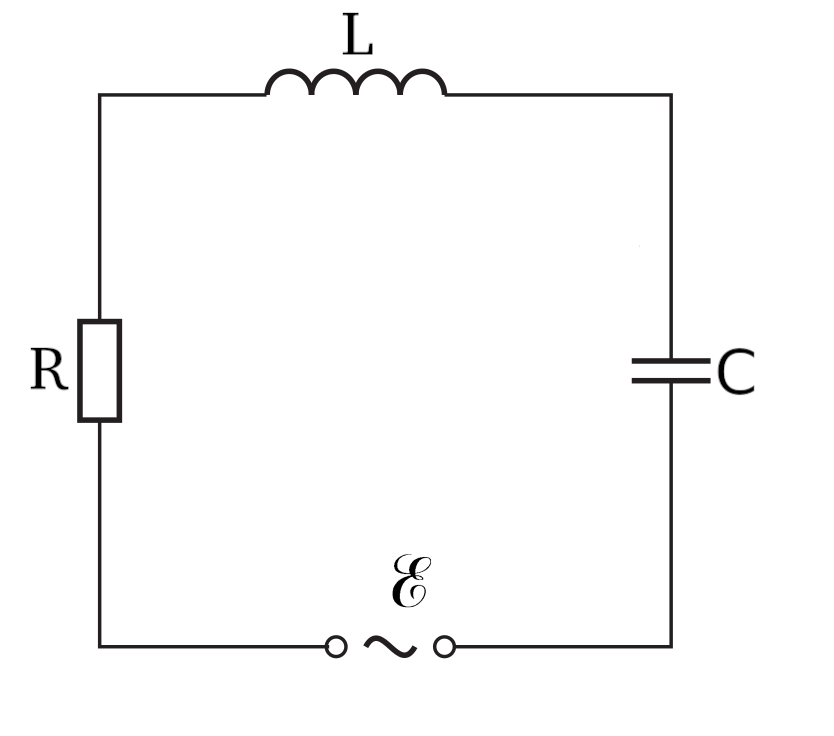
\includegraphics[width=0.2\textwidth]{../res/seq_osc_circ.png}
	\caption{Последовательный колебательный контур}
	\label{fig:seq_osc_circ}
\end{wrapfigure}

Рассмотрим последовательный колебательный контур без источника ЭДС (рис. $\ref{fig:seq_osc_circ}$).  Пусть напряжение на конденсаторе меняется по закону $U = U(t)$. Тогда, согласно второму правилу Кирхгофа, сумма падений напряжений равна 0:
$$
L \frac{dI}{dt} + U + RI = 0
$$
Ток через конденсатор определяется из соотношения
$$
I = \frac{dq}{dt} = C\frac{dU}{dt}
$$
Тогда получим дифференциальное уравнения второго порядка, описывающее \textit{свободные колебания} в линейной системе:
$$
LC \frac{d^2 U}{dt^2} + RC \frac{dU}{dt} + U = 0
$$
Данное уравнение можно переписать в виде:
\begin{equation*}
	\ddot{U} + 2\gamma \dot{U} + \omega_0^2 U = 0
	\label{eq:diff_eq}
\end{equation*}
где введены обозначения $\gamma = \frac{R}{2L}$ -- \textit{коэффициент затухания}, $\omega_0 = \frac{2\pi}{T_0} = \frac{1}{\sqrt{LC}}$ -- \textit{собственная частота} колебательной системы, $T_0 = 2\pi \sqrt{LC}$ -- \textit{период собственных колебаний}.

Найдём решение однородного дифференциального уравнения с постоянными коэффициентами. Запишем характеристическое уравнение:
$$
\lambda^2 + 2\gamma \lambda + \omega_0^2 = 0
$$
$$
D_1 = \frac{D}{4} = \gamma^2 - \omega_0^2
$$
В зависимости от знака дискриминанта квадратного уравнения возможны три случая.

\begin{enumerate}
	\item \textit{Затухающие колебания}.
	
	Рассмотрим случай, когда $D_1 < 0$. Тогда $0 < \gamma < \omega_0$, что эквивалентно
	$$
	0 < R < 2 \sqrt{\frac{L}{C}} = R_{кр}
	$$
	Сопротивление $R_{кр} = 2 \sqrt{\frac{L}{C}}$ называется критическим, а $\rho = \sqrt{\frac{L}{C}}$ -- волновым.
	
	В рассматриваемом случае характеристическое уравнение имеет два комплексных корня 
	$$
	\lambda_{1,2} = -\gamma \pm j\sqrt{\omega_0^2 - \gamma^2}
	$$
	Величину $\omega = \sqrt{\omega_0^2 - \gamma^2}$ называют частотой свободных колебаний. Решением уравнения будет
	$$
	U(t) = U_1 \cdot e^{-\gamma t} \cdot e^{-j\omega t} + U_2 \cdot e^{-\gamma t} \cdot e^{j\omega t}
	$$
	где $U_1$ и $U_2$ -- произвольные постоянные.
	
	Полученное уравнение можно представить в виде
	\begin{equation*}
		U(t) = U_0 e^{-\gamma t} sin(\omega t + \varphi_0)
		\label{eq:damp_osc}
	\end{equation*}
	Данное уравнение является гармоническим с фазой $\omega t + \varphi_0$ и экспоненциально убывающей амплитудой $U_0 e^{-\gamma t}$.
	
	График зависимости напряжения от времени представлен на рисунке $\ref{fig:damp_osc}$.
	
	\begin{figure}[H]
		\vspace{-10pt}
		\centering
		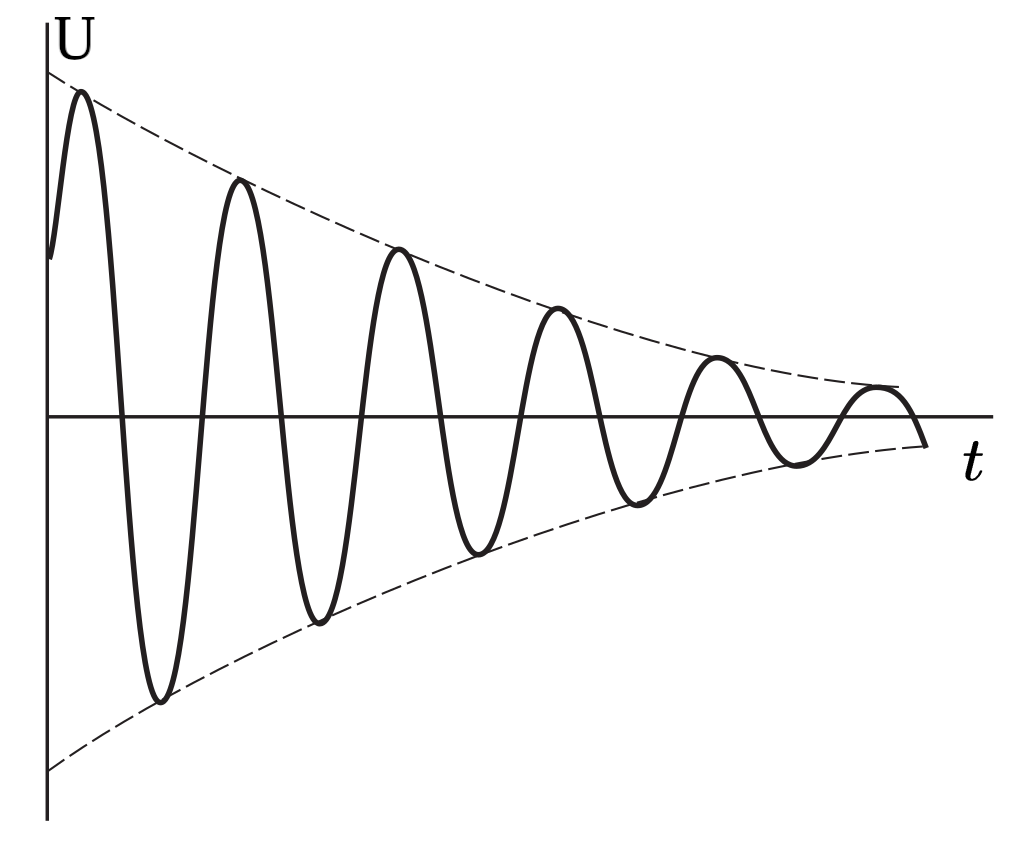
\includegraphics[width=0.3\textwidth]{../res/damp_osc.png}
		\caption{Затухающие колебания}
		\label{fig:damp_osc}
	\end{figure}

	С точки зрения математики данный колебательный процесс не периодичен. Тем не менее функция $U(t)$ обращается в ноль или достигает экстремумов через один и тот же промежуток времени, который называю \textit{периодом затухающих колебаний}.
	
	\item \textit{Критический режим}. 
	
	Рассмотрим случай, когда $D_1 = 0$. Тогда 
	$$
	\gamma = \omega_0
	$$
	Характеристическое уравнение имеет один корень
	$$
	\lambda = - \gamma
	$$
	Решением исходного уравнения будет
	$$
	U(t) = U_0 e^{-\gamma t}
	$$
	где $U_0$ -- постоянная, определяемая из начальных условий.
	
	Заметим, что данный режим физически не реализуем, так как равенство $\gamma = \omega_0$ не может быть выполнено точно. Данный случай нужно рассматривать как переходный между затухающими колебаниями и апериодическим режимом.
	
	\item \textit{Апериодический режим}. 
	
	Рассмотрим случай, когда $D_1 > 0$. Тогда $0 < \omega_0 < \gamma$. Характеристическое уравнение имеет два действительных корня
	$$
	\lambda_{1,2} = -\gamma \pm \sqrt{\omega_0^2 - \gamma^2}
	$$
	Решением дифференциального уравнения будет
	$$
	U(t) = e^{-\gamma t} \cdot (U_1 e^{-j\omega t} + U_2 e^{j\omega t})
	$$
	где $U_1$ и $U_2$ -- произвольные постоянные.
\end{enumerate}

\subsection*{Характеристики затухающих колебаний}

Важными характеристиками колебательных систем являются добротность $Q$ и логарифмический декремент $d$.

Логарифм отношения амплитуд колебаний в двух последовательных максимумах называется логарифмическим декрементом
$$
d = \ln{\left(\frac{A_n}{A_{n+1}}\right)}
$$
Определив положения последовательных максимумов из формулы $\ref{eq:damp_osc}$, можно получить следующее соотношение
\begin{equation*}
	d = \gamma T
	\label{eq:log_dec}
\end{equation*}
где $T$ -- период затухающих колебаний.

\textit{Постоянной времени затухания} $\tau$ называется время, за которое амплитуда колебаний убывает в $e$ раз. Коэффициент затухания и постоянная времени связаны соотношением
\begin{equation*}
	\tau = \frac{1}{\gamma}
	\label{eq:const_time}
\end{equation*}

Из уравнений $\ref{eq:log_dec}$ и $\ref{eq:const_time}$ следует, что логарифмический декремент можно определить как число полных колебаний $N = \frac{\tau}{T}$ за время затухания $\tau$:
$$
d = \frac{1}{N}
$$

Добротностью колебательной системы $Q$ называется
$$
Q \equiv \frac{\pi}{d} = \frac{\pi}{\gamma T} = \frac{\omega}{2 \gamma}
$$ 
Чем выше добротность колебательной системы, тем меньше будут потери энергии. Докажем данное утверждение.

Амплитуда колебаний напряжение за период уменьшается в $e^{\gamma T}$ раз. Полная энергия системы $W$ определяется как максимальная энергия электрического поля конденсатора или магнитного поля индуктивности
$$
W = \frac{CU^2}{2} = \frac{LI^2}{2}
$$
Из этого соотношения видно, что за период энергия системы уменьшается как квадрат амплитуды в $e^{2\gamma T}$ раз.
Тогда потери энергии системы равно
$$
\Delta W = W(t_0) - W(t_0 + T) = (1 - e^{-2\gamma T}) W(t_0)
$$
Если затухание мало, то есть $\gamma T \ll 1 \Rightarrow Q \gg 1$, то экспоненту можно разложить по формуле Тейлора
$$
\Delta W \approx 2 \gamma T W
$$
$$
\frac{W}{\Delta W} = \frac{1}{2\gamma T} = \frac{1}{2\pi}Q
$$
Таким образом, добротность с энергетической точки зрения определяет отношении энергии системы к потерям за период.

\subsection*{Вынужденные колебания}

Если в цепь последовательного колебательного контура включен гармонический источник ЭДС $\varepsilon(t) = \varepsilon_0 \cos{(\omega t)}$, то
$$
\ddot{U} + 2\gamma \dot{U} + \omega_0^2 U = \frac{\varepsilon_0}{LC} \cos{(\omega t)}
$$
Решением неоднородного дифференциального уравнения будет сумма однородного и частного решений
$$
U_{общ}(t) = U_{одн}(t) + U_{част}(t)
$$
Решением однородного уравнения будут затухающие колебания
$$
U_{одн}(t) = U_0 e^{-\gamma t} sin(\omega t + \varphi_0)
$$
Частное решение неоднородного уравнения будем искать в виде:
$$
U_{част}(t) = A e^{j \omega t}
$$
Неоднородность уравнения в комплексной форме равна
$$
\varepsilon = \frac{\varepsilon_0}{LC}e^{j \omega t}
$$
Подставив частное решение в исходное уравнение находим
$$
U_{част}(t) = \frac{\varepsilon_0 e^{j \omega t}}{LC (\omega_0^2 + 2 j \gamma \omega  - \omega^2)}
$$
Решением является только действительная часть, тогда
$$
U_{част}(t) = \frac{\varepsilon_0}{LC} \frac{1}{\sqrt{(\omega_0^2 - \omega^2)^2 + 4 \omega^2 \gamma^2 }} \cos{\left(\omega t - \arctg{\frac{2 \omega \gamma}{\omega_0^2 - \omega^2}}\right)}
$$
Итого уравнением вынужденных колебаний будет
$$
U(t) = U_0 e^{-\gamma t} sin(\omega t + \varphi_0) +  \frac{\varepsilon_0}{LC} \frac{1}{\sqrt{(\omega_0^2 - \omega^2)^2 + 4 \omega^2 \gamma^2 }} \cos{\left(\omega t - \arctg{\frac{2 \omega \gamma}{\omega_0^2 - \omega^2}}\right)}
$$
Заметим, что амплитуда однородного решения убывает экспоненциально, а амплитуда частного решения остается постоянной. Поэтому, через большой промежуток времени, напряжение будет изменяться по закону $U(t) \approx U_{част}(t)$. Итого, установившимися вынужденными колебаниями будут гармонические колебания с частотой вынуждающей ЭДС.

\subsection*{Резонанс в параллельном колебательном контуре}

Рассмотрим параллельный колебательный контур. Пусть к нему подключен идеальный источник ЭДС, обладающий бесконечно большим внутренним сопротивлением, задающий во внешней цепи ток, изменяющийся по гармоническому закону $I = I_0 \cos{\left(\omega t + \phi_0\right)}$.

\begin{figure}[H]
	\vspace{-10pt}
	\centering
	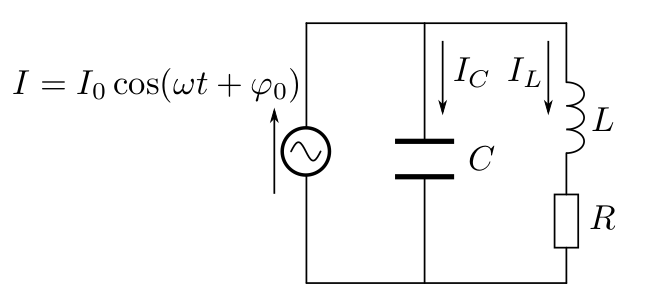
\includegraphics[width=0.4\textwidth]{../res/parallel_contour.png}
	\caption{Параллельный колебательный контур}
	\label{fig:parallel_contour}
\end{figure}

Методом комплексных амплитуд определим зависимости напряжения и тока на элементах цепи:
\begin{equation*}
	\begin{split}
		I_C &= I_0 \frac{1 + j \frac{\rho \omega}{R \omega_0}}{1 + j \frac{\rho}{R} \left( \frac{\omega}{\omega_0} - \frac{\omega_0}{\omega} \right) } \\
		I_L &= I_0 \frac{-j \frac{\rho \omega_0}{R \omega}}{1 + j \frac{\rho}{R}\left(\frac{\omega}{\omega_0} - \frac{\omega_0}{\omega}\right)} \\
		U_C &= I_0 \frac{\rho^2}{R} \frac{1-j \frac{\rho \omega_0}{R \omega}}{1 + j \frac{\rho}{R}\left(\frac{\omega}{\omega_0} - \frac{\omega_0}{\omega}\right)}
	\end{split}
\end{equation*}

Далее будем рассматривать высокодобротный колебательный контур вблизи резонансной частоты $Q \approx \frac{\rho}{R} \gg 1$. Тогда выражения для токов примут вид:
\begin{equation*}
	\begin{split}
		I_C &= Q I_0 \frac{\omega}{\omega_0} \frac{ \cos \left( \omega t - \varphi_C \right) }{ \sqrt{1 + (\tau \Delta \omega)^2} } \\
		I_L &= Q I_0 \frac{\omega_0}{\omega} \frac{ \cos \left( \omega t - \varphi_L \right) }{ \sqrt{1 + (\tau \Delta \omega)^2} } \\
		U_C &= Q \rho I_0 \frac{ \cos \left( \omega t - \varphi_U \right) }{ \sqrt{1 + (\tau \Delta \omega)^2} }		
	\end{split}
\end{equation*}
Фазы токов определяются по формулам:
\begin{equation*}
	\begin{split}
		\varphi_C &= \arctg{\left(\tau \Delta \omega\right)} - \frac{\pi}{2} + \frac{1}{Q} \\
		\varphi_L &= \arctg{\left(\tau \Delta \omega\right)} + \frac{\pi}{2} \\
		\varphi_U &= \arctg{\left(\tau \Delta \omega\right)} + \frac{\omega_0}{\omega} \frac{1}{Q} \\
	\end{split}
\end{equation*}

При резонансе $\omega = \omega_0$, $\Delta \omega = 0$ и формулы можно упростить:
\begin{equation*}
	\begin{split}
		I_C &= Q I_0 \cos \left( \omega_0 t - \varphi_C \right) \\
		I_L &= Q I_0 \cos \left( \omega_0 t - \varphi_L \right) \\
		U_C &= Q^2 R I_0 \cos \left( \omega_0 t - \varphi_U \right) \\		
		\varphi_C &= -\frac{\pi}{2} + \frac{1}{Q} \\
		\varphi_L &= \frac{\pi}{2} \\
		\varphi_U &= \frac{1}{Q} \\
	\end{split}
\end{equation*}

Из полученных соотношений следует, что ток через конденсатор $I_C$ опережает внешний ток по фазе на $\frac{\pi}{2} - \frac{1}{Q} \approx \frac{\pi}{2}$. Ток через катушку индуктивности отстает от внешнего тока по фазе на $\frac{\pi}{2}$. Напряжение на конденсаторе отстает от внешнего тока по фазе на $\frac{1}{Q}$.

Ток через индуктивность и конденсатор в $Q$ раз больше внешнего тока. Поэтому резонанс в последовательном колебательном контуре называют \textit{резонансном токов}.

С помощью полученных соотношений не трудно построить векторную диаграмму.

\begin{figure}[H]
	\vspace{-10pt}
	\centering
	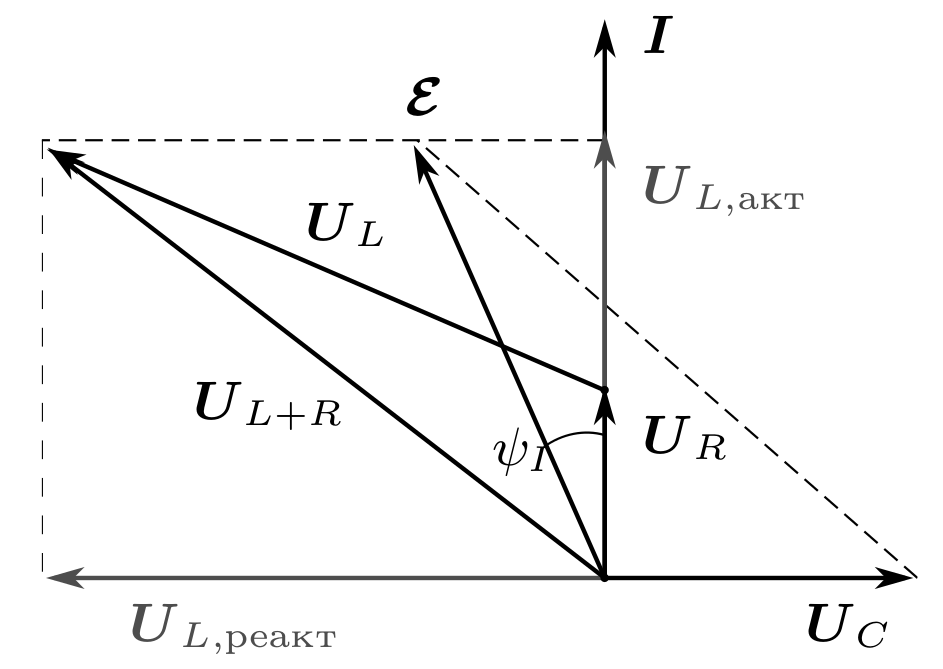
\includegraphics[width=0.4\textwidth]{../res/vect_diagram.png}
	\caption{Векторная диаграмма при резонансе токов}
	\label{fig:vect_diagram}
\end{figure}
	
	\newpage
	
	\section*{Схема экспериментальной установки}

Схема экспериментальной установки изображена на рисунке:

\begin{figure}[H]
	\centering
	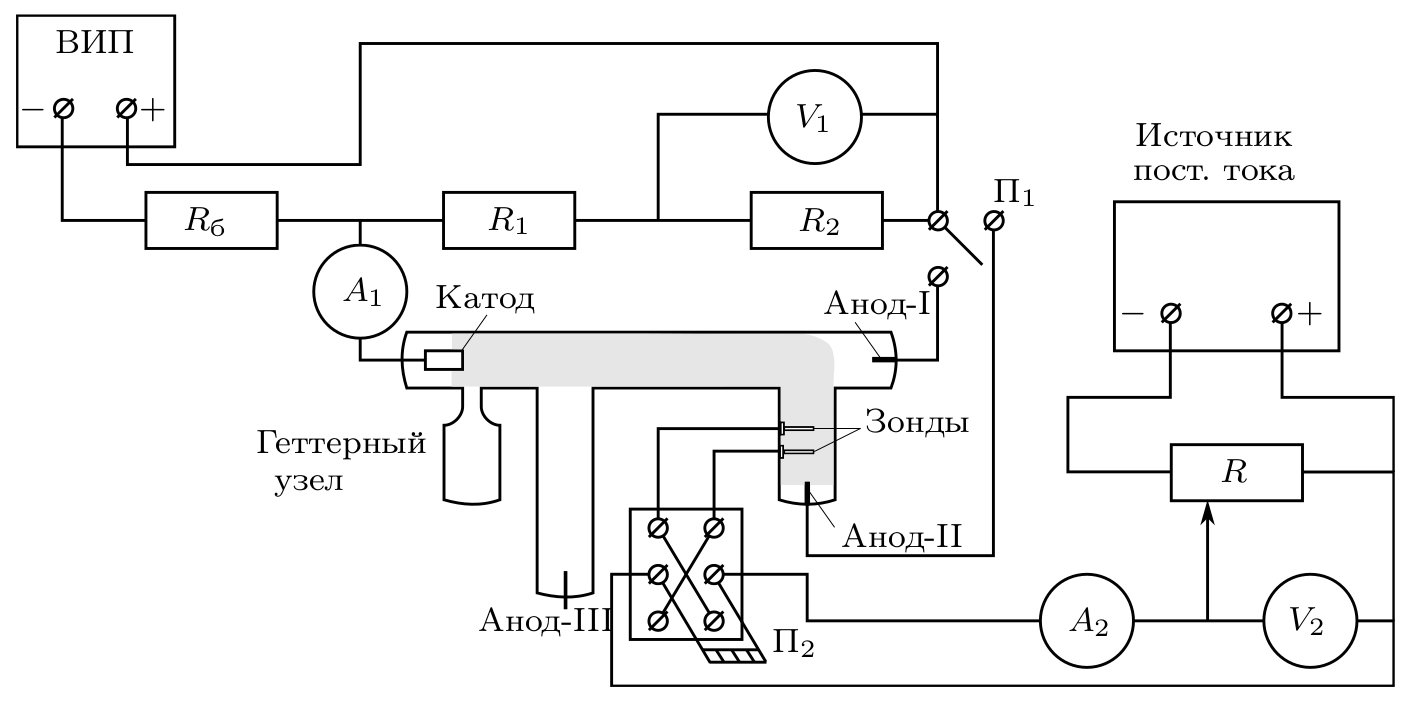
\includegraphics[width=1\textwidth]{../res/exp scheme.png}
\end{figure}

Установка состоит из стеклянной газоразрядной трубки, в которой находится катод и три анода. В данной работе анод 3 не используется. Трубка наполнена изотопом неона $^{22}Ne$ при давлении 2 мм рт.ст. Катод и один из анодов с подключаются к высоковольтному источнику питания (ВИЧ) через балластный резистор $R_б \approx 450 \dim кОм$. Анод 1 и 2 можно подключать к ВИЧ через переключатель $П_1$. Миллиамперметр $А_1$ измеряет ток между анодом и катодом, а цифровой вольтметр $V_1$ измеряет напряжение в газоразрядной трубке. Вольтметр $V_1$ подключен через делитель напряжения с коэффициентом $K = 10$. 

Во второй части работы исследуются характеристики плазмы с помощью двух зондов. Зонды изготовлены из молибденовой проволоки диаметром $d = 0,2 \dim мм$, длиной $l = 5,2 \dim мм$. С помощью источника постоянного тока на зонды подается ток, который измеряется миллиамперметром $A_2$. Напряжение на зондах измеряется вольтметром $V_2$. Для регулировки напряжения используется реостат $R$.


	
	\section*{Оборудование}

\begin{enumerate}
	\item Генератор звуковой частоты.
	
	\item Вольтметр.
	
	\item Амперметр.
	
	\item Электронный осциллограф.
	
	\item Измерительная катушка.
	
	\item Медный цилиндр.
\end{enumerate}
	
	\section*{Экспериментальные результаты}

Оценим значение частоты $nu_h$, при котором скиновая длина равна толщине стенок экрана $h = 1.5$ мм, приняв значение проводимости медного экрана $\sigma = 5 \cdot 10^7 \; \text{См}/\text{м}$.
$$ \nu_h = \frac{1}{\pi \sigma \mu_0 h^2} = 2250 \; \text{Гц}. $$ 

Исследование полей проведем в трех диапазонах частот $\nu$: низкие ($0.01 \nu_h \div 0.05 \nu_h$), средние ($0.05 \nu_h \div 0.5 \nu_h$) и высокие ($0.5 \nu_h \div 15 \nu_h$).

\subsection*{Низкие частоты}

Согласно $\ref{eq:UInu}$ соотношение между полем внутри $H_1$ и полем снаружи $H_0$ зависит от тока в катушке и напряжения на вольтметре. Введем обозначения $\xi = \frac{U}{\nu I}$ и $\xi_0: \xi = \xi_0 \cdot \frac{H_1}{H_0}$. 

При малых частотах толщина скин-слоя больше толщины стенок экрана, выполняется приближение \ref{eq:low_ampl}. Тогда
$$\frac{1}{\xi^2} = \frac{1}{\xi_0^2} + \left(\frac{ah\mu_0 \sigma \pi \nu}{\xi_0}\right)^2.$$

Построим график $\frac{1}{\xi^2}(\nu^2)$.

\begin{figure}[H]
	\centering
	\includegraphics{../gen/xi-2_nu2.pdf}
	\caption{Зависимость $\frac{1}{\xi^2}$ от частоты тока $\nu^2$}
	\label{fig:xi-2_nu2}
\end{figure}

Найдем параметры графика $y = kx + b$ по методу наименьших квадратов. По ним определим $\xi_0 = 0.0154$ и проводимость фильтра $\sigma = \frac{\sqrt{k} \xi_0}{a h \mu_0 \pi} = 2.17 \cdot 10^7 \; \frac{\text{См}}{\text{м}}$.

\subsection*{Средние частоты}

Для данного диапазона частот мы можем определить сдвиг фаз между $U$ и $I$, определяемый \ref{eq:low_phase}. 

Построим график $\tan \psi (\nu)$.

\begin{figure}[H]
	\centering
	\includegraphics{../gen/tanpsi_nu.pdf}
	\caption{Зависимость $\tan \psi$ от частоты тока $\nu$}
	\label{fig:tanpsi_nu}
\end{figure}

Линейность зависимости быстро исчезает, однако этого достаточно для еще одной оценки проводимости $\sigma = \frac{k}{a h \mu_0 \pi} = 2.41 \cdot 10^7 \; \frac{\text{См}}{\text{м}}$.

\subsection*{Высокие частоты}

Для данного диапазона выполняется приближение \ref{eq:high_phase}.

Построим график $(\psi - \frac{\pi}{4}) (\frac{1}{\sqrt{\nu}})$.

\begin{figure}[H]
	\centering
	\includegraphics{../gen/psi_nu.pdf}
	\caption{Зависимость $\psi - \frac{\pi}{4}$ от частоты тока $\sqrt{\nu}$}
	\label{fig:psi_nu}
\end{figure}

Оценим проводимость $\sigma = \frac{k^2}{h^2 \mu_0 \pi}= 3.91 \cdot 10^7 \; \frac{\text{См}}{\text{м}}$.
Значение проводимости в данной серии измерений значительно отличается от остальных $\sigma$.

\subsection*{Индуктивность}

Измерим индуктивность фильтра с помощью RLC-метра. 

\begin{figure}[H]
	\centering
	\includegraphics{../gen/L_nu.pdf}
	\caption{Зависимость $L$ от частоты тока $\nu$}
	\label{fig:L_nu}
\end{figure}

Согласно \ref{eq:LL_nu^2} построим линеаризованный график.

\begin{figure}[H]
	\centering
	\includegraphics{../gen/psi_nu.pdf}
	\caption{Зависимость $(L_{max} - L_{min})/(L - L_{min})$ от частоты тока $\nu^2$}
	\label{fig:LL_nu^2}
\end{figure}

Определим проводимость $\sigma = \frac{\sqrt{k}}{a h \mu_0 \pi} = 1.99 \cdot 10^7 \; \frac{\text{См}}{\text{м}}$.

\subsection*{Общие результаты}

Сведем результаты в один график. Для этого построим экспериментальный график по всем значениям, собранным в работе, а также построим теоретические графики по \ref{eq:solution} для измеренных $\sigma$.

\begin{figure}[H]
	\centering
	\includegraphics{../gen/summary.pdf}
	\caption{Зависимость $(L_{max} - L_{min})/(L - L_{min})$ от частоты тока $\nu^2$}
	\label{fig:summary}
\end{figure}

Как можно видеть, экспериментальные точки хорошо сходятся с теоретическими кривыми для $\sigma \approx 2 \cdot 10^7  \; \frac{\text{См}}{\text{м}}$.
	
	\newpage
	
	\section*{Заключение и выводы}

Данная работа демонстрирует точность модели спектрального анализа, описывающей структуру различных сигналов. С помощью спектрального анализа можно вычислить реакцию линейной стационарной системы на произвольный периодический сигнал как сумму реакций на его гармонические составляющие, что сильно упрощает расчеты.
	
\end{document}